\chapter{Minimum Deviation Angle}

\section{Aim}
To determine the angle of minimum deviation of a triangular prism

\section{Background Information}
When a ray of light passes through a glass prism it tends to bend away from its original direction. The deviation angle is the angle between the original path of the light and the final path of the light after leaving the prism. What is the relationship between the angle of incidence and the minimum angle of deviation?

\section{Materials}
Triangular prism ($60^\circ$), 4 optical pins, 4 drawing pins, drawing body, ruler, protractor,  pencil, white sheet of paper, graph paper.

\section{Procedure}
\begin{enumerate}
\item Fix a white sheet of paper on a soft drawing board by using the drawing pins, and place a triangular glass prism on the white sheet of paper.
\item Trace the boundaries of the prism by using a sharp pencil and label the vertices as A, B and C.
\item Remove the glass prism and mark a point P along the line just above the center of side AB (see figure).
\item Draw a normal line MPN to line AB and construct another line XP such that the incident angle $i=30^\circ$.
\item Replace the glass prism to its original position and erect two pins Q$_1$ and Q$_2$ along line XP, then view the images of these pin from side BC.
\item Erect the other two pins Q$_3$ and Q$_4$ so that they appear inline with Q$_1$ and Q$_2$.
\item Remove the glass prism and draw a line through the point Q$_3$ and Q$_4$ to meet BC at R.
\item Extend lines XP and Q$_3$R to meet at point K using dotted lines.
\item Measure the angle of deviation, $d$, as seen in the figure. 
\item Repeat the experiment by increasing the angle of incidence by intervals of $5^\circ$ to obtain five more readings, tabulate your results.
\end{enumerate}

\begin{figure}[h!]
\centering
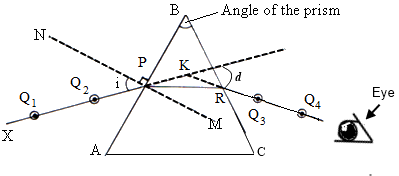
\includegraphics[width=10cm]{./img/minimum-deviation-1.png}
\caption{Minimum Deviation Angle practical setup}
\label{fig:minimum-deviation-1}
\end{figure}

\section{Safety Measure}
The glass prism should be clean.

\section{Analysis and Interpretation}
\begin{enumerate}
\item Draw the graph $d$ against $i$.
\item What happens to the deviation angle when the angle of incidence increases?
\item What is the nature of the graph?
\item From the graph explain how the minimum angle of deviation can be found.
\end{enumerate}

\section{Conclusion}
From the graph, what is the value of the minimum angle of deviation?

\section{Questions for Discussion}
\begin{enumerate}
\item Why is the incident ray deviated when it leaves the surface AB of the glass prism?
\item How can this experiment be used to find the refractive index of the glass prism?
\end{enumerate}

\section{Reflection and Self Assessment}
\begin{enumerate}
\item Did you have any difficulties when performing this experiment? Explain.
\item Which parts of the experiment did you find most interesting? Explain.
\item What is a common observation that is related to this glass prism experiment?
\end{enumerate}